\chapter{Tromba Marina}\label{ch:tromba}
This chapter provides an extended summary for the physical model presented in the paper ``Real-time Implementation of a Physical Model of the Tromba Marina'' \citeP[D] and used in the paper ``Resurrecting the Tromba Marina: A Bowed Virtual Reality Instrument using Haptic Feedback and Accurate Physical Modelling'' \citeP[E]. After a brief introduction of the tromba marina, and summarising the physical model -- with reference to the theory explained in the previous parts of this thesis -- this chapter elaborates on the contents of paper \citeP[D] by providing more details on the implementation. As much as possible, this chapter follows the notation of paper \citeP[D], as long as it is coherent with what has already been presented in this thesis. Discrepancies between this chapter and the paper will be clearly highlighted. 

\section{Introduction}
The tromba marina is a bowed monochord instrument from medieval Europe (see Figure \ref{fig:tromba}). It has a long quasi-trapezoidal body and is unique due to its oddly-shaped bridge that the string rests on. The bridge is often called a `shoe' due to its shape and is free to rattle against the body in sympathy with the movement of the vibrating string (see Figure \ref{fig:bridge}). This rattling causes a sound with brass or trumpet-like qualities, hence the name \textit{tromba} which stems from the Italian word trumpet. The rarity of the instrument as well as its interesting physics makes it an ideal case for a physical modelling implementation.

\begin{figure}
    \centering
    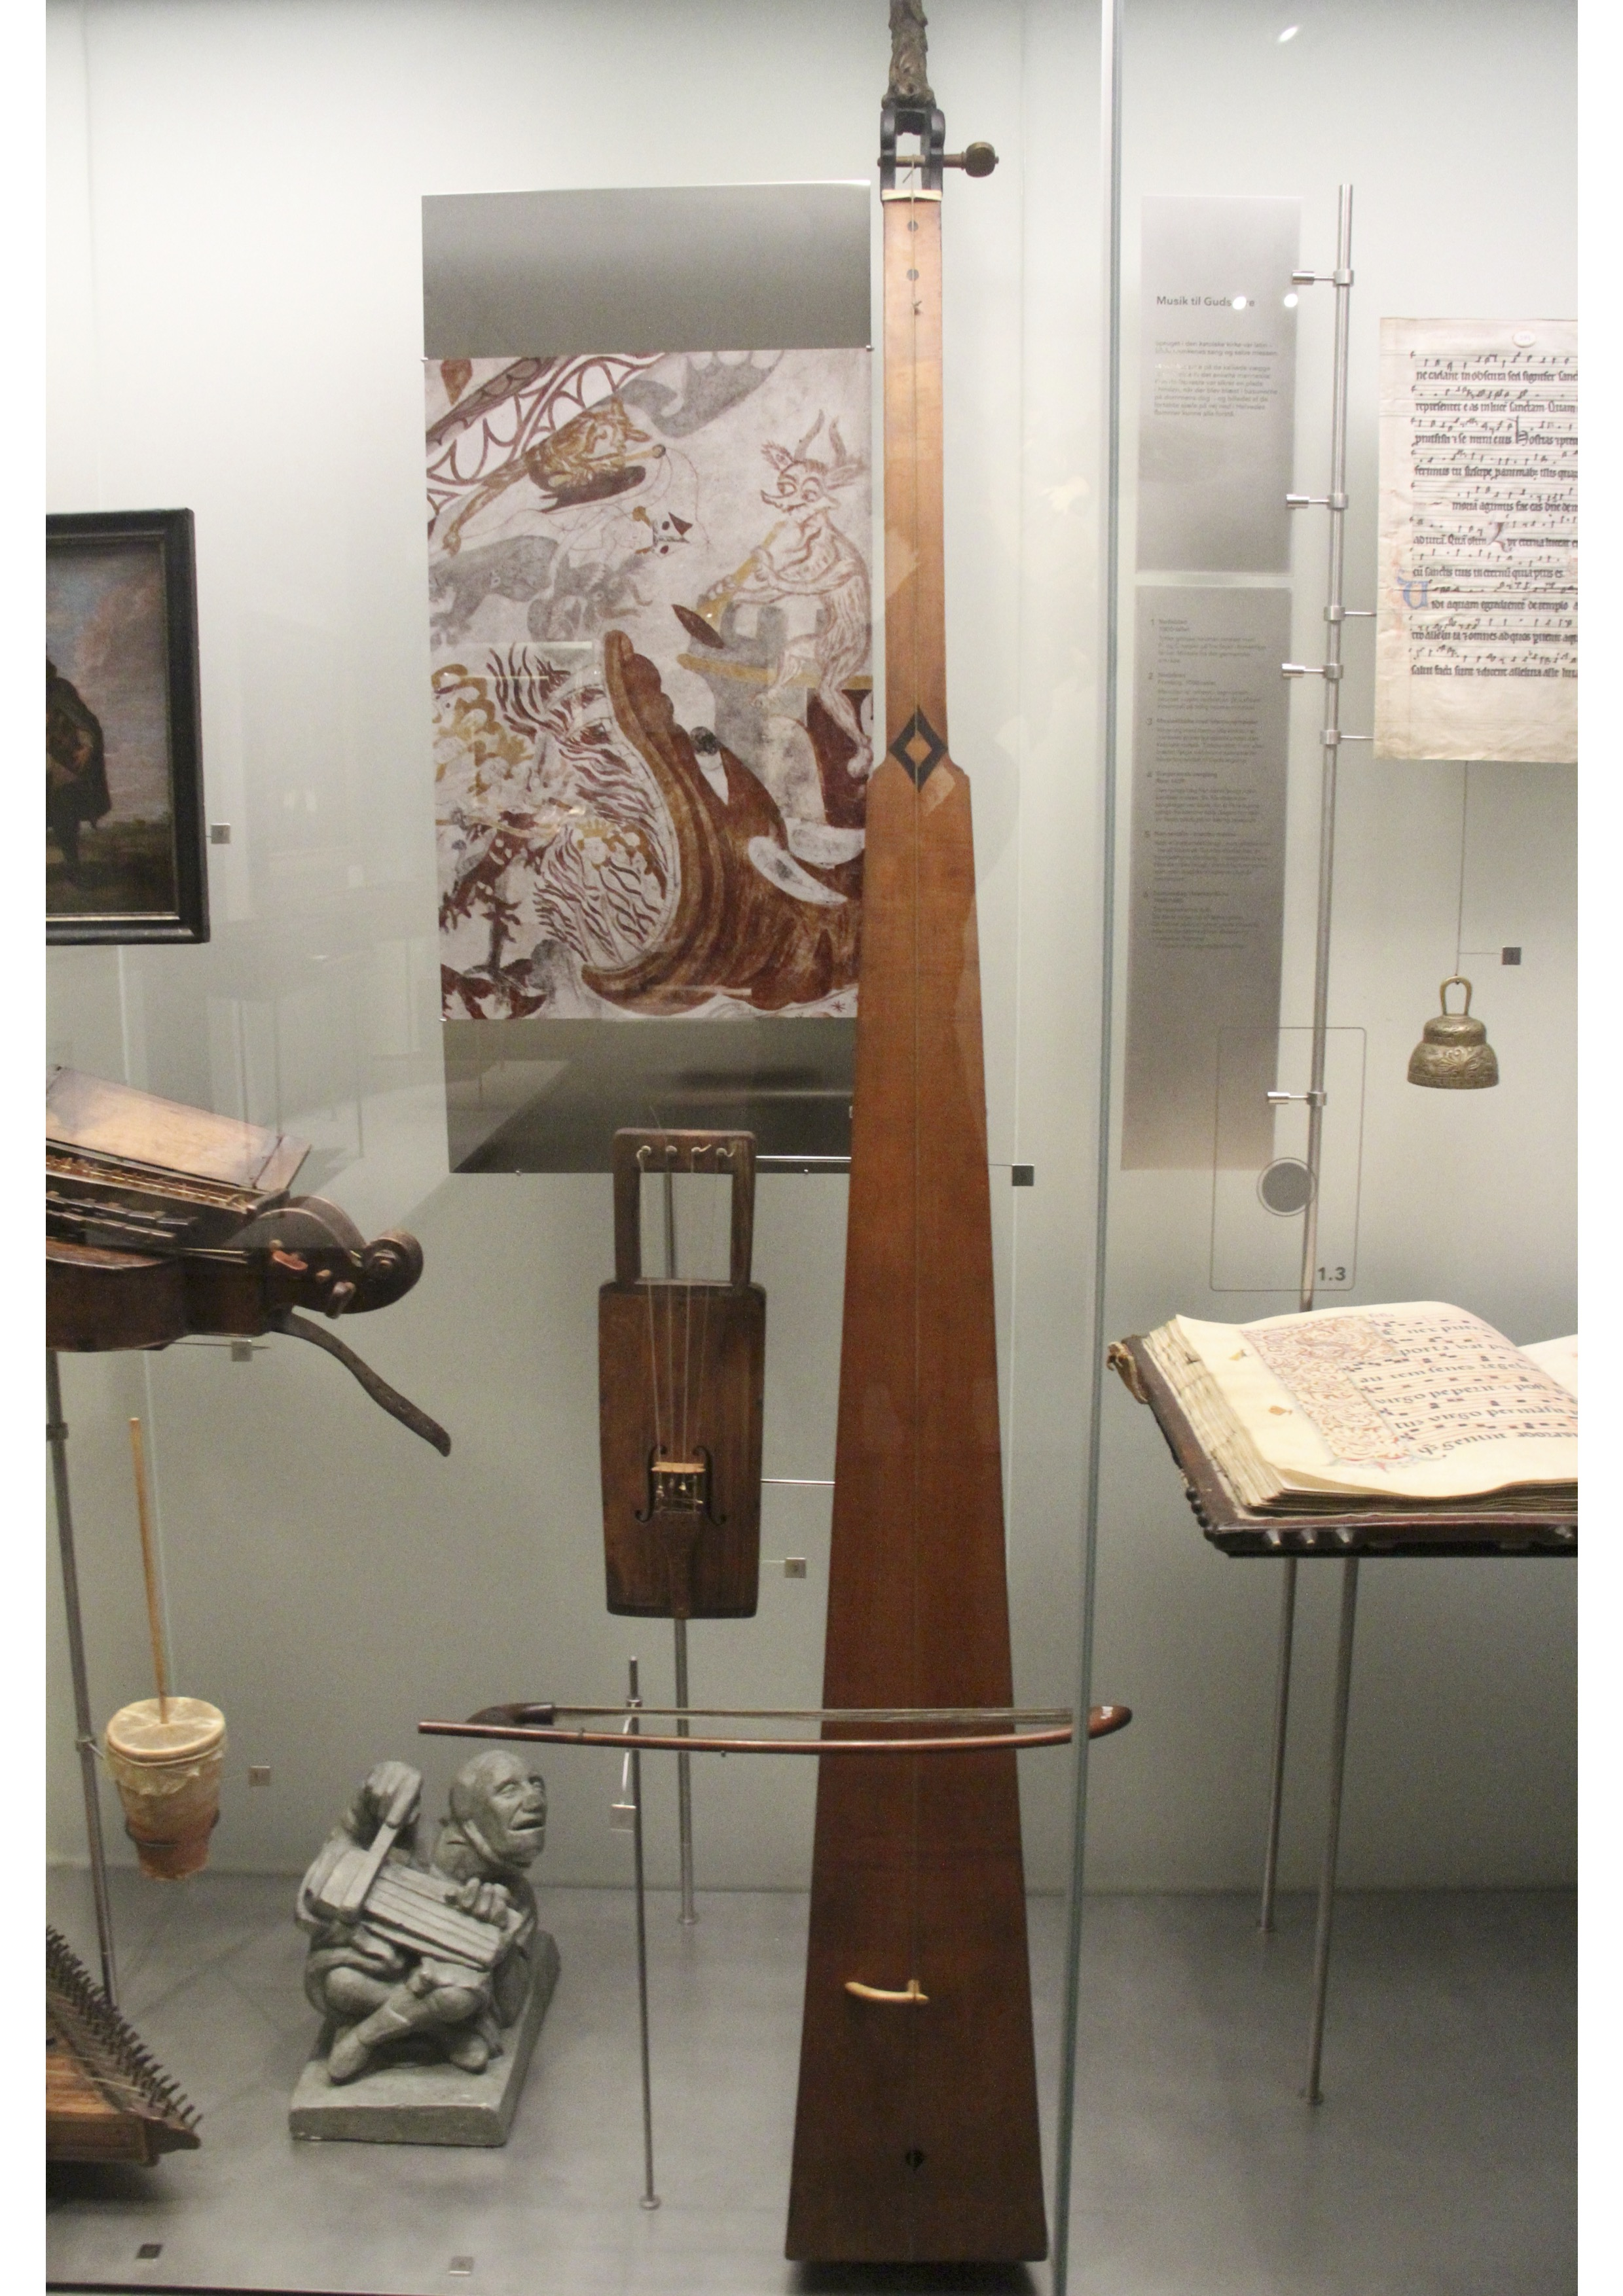
\includegraphics[width=0.5\textwidth]{figures/contributions/tromba/IMG_7980.pdf}
    \caption{The tromba marina from the Danish Music Museum in Copenhagen. (As shown in paper \citeP[D].)}
\label{fig:tromba}
\end{figure}
  
\begin{figure}
    \centering
    \includegraphics[width=0.8\textwidth]{figures/contributions/tromba/IMG_7982.JPG}
    \caption{The bridge of the tromba marina from the Danish Music Museum in Copenhagen. The right side of the bridge is pressed against the body by the string while the left side is free and can rattle against the body. (As shown in paper \citeP[D].)}
\label{fig:bridge}
\end{figure}

\section{Physical Model}
The full musical instrument has been divided into three parts: the string, the bridge and the body each of which will briefly be presented here on. 
\subsection{Continuous Time}
Each component in isolation is of the form 
\begin{equation}\label{eq:trombaPDEForm}
    \L q = 0
\end{equation}
where $\L$ is a linear (partial) differential operator and $q(\boldsymbol{x}, t)$ describes the state of the component in isolation. $q$ is defined for time $t\geq 0$ and spatial coordinate $\boldsymbol{x}\in \D$ where the dimensions of domain $\D$ depend on the dimensions of the system at hand. Using the form in Eq. \eqref{eq:trombaPDEForm} allows for a much more compact notation later on. In the following, subscripts `s', `m' and `p' will be used to denote the `string', `bridge' (mass), and `body' (plate) respectively.

\subsubsection{String}
The string of the tromba marina is modelled as a damped stiff string of length $L$ (in m) (see Chapter \ref{ch:stiffString}). With reference to the form in \eqref{eq:trombaPDEForm}, its transverse displacement is described by $q = u(\chi, t)$ (in m) and is defined for $\chi \in \D_\stxt$ where domain $\D_\stxt = [0, L]$.\footnote{Notice that $\chi$ rather than $x$ is used here. As $x$ will be used as a spatial coordinate for the body later on, a different symbol is used for the string to differentiate between different coordinate-systems.} Using partial differential operator $\L = \L_\text{s}$, the PDE describing its motion is defined as
\begin{equation}\label{eq:trombaStiffString}
    \L_\stxt u =  0,
\end{equation}
where (see Eq. \eqref{eq:stiffStringPDE})
\begin{equation*}
    \L_\stxt = \rho_\stxt A \ptt - T\partial_\chi^2 + E_\text{s}I\partial_\chi^4+2\rho_\stxt A\szX[\stxt]\pt-2\rho_\stxt A\soX[\stxt]\pt\partial_\chi^2\ .
\end{equation*}
The parameters are as defined for Eq. \eqref{eq:stiffStringPDE} with the possible addition of the `s' subscript.
Compared to the schemes presented in previous chapters, using a partial differential operator to combine all operators like this, is purely different from a notational point of view, and does not change the behaviour of the system. If Eq. \eqref{eq:trombaStiffString} is expanded and all terms except for $\rho_\stxt A \ptt$ are moved to the right-hand side, one arrives again at the damped stiff string PDE in Eq. \eqref{eq:stiffStringPDE}.

As the string is bowed, one can extend the PDE in \eqref{eq:trombaStiffString} can be extended to 
\begin{equation}
    \L_\stxt u =  - \delta(\chi-\chi_\text{B})F_\text{B}\Phi(\vrel),
\end{equation}
with bow position $\chi_\text{B} = \chi_\text{B}(t) \in \D_\stxt$ (in m), bow force $F_\text{B} = F_\text{B}(t)$ and relative velocity between the bow and the string $\vrel=\vrel(t)$. The static friction model in Eq. \eqref{eq:staticFriction} has been chosen for simplicity. For more details on this bow model, see Section \ref{sec:staticFricMod}.

\subsubsection{Bridge}
The bridge is modelled using a mass-spring-damper system (see Section \ref{sec:massSpringDamping}). With reference to Eq. \eqref{eq:trombaPDEForm}, the transverse displacement of the mass is described by $q = w(t)$ (in m) and using differential operator $\L = \L_\text{m}$ its PDE is 
\begin{equation}
    \L_\text{m} w = 0
\end{equation}
where (see Eq. \eqref{eq:massSpringDampingPDE})
\begin{equation*}
    \mathcal{L}_\text{m}=M\frac{d^2}{dt^2}+M\omega_0^2+M\sigma_\text{m}\frac{d}{dt}.
\end{equation*}
Here, $\omega_0 = \sqrt{K/M}$ (in s$^{-1}$) and $\sigma_\text{m} = R/M$ (in s$^{-1}$) and other parameters are as in Eq. \eqref{eq:massSpringDampingPDE}.\footnote{In paper \citeP[D], the symbol $R$ is used for the damping coefficient, but for coherence in this work, $\sigma_\text{m}$ is used instead.} 

Notice that when using a differential operator for an ODE, the dots to denote a temporal derivative (as e.g. Eq. \eqref{eq:massSpringDampingPDE}) need to be written in an operator form. Here, Leibniz's notation is chosen (see Section \ref{sec:differentialEquations}). 


\subsubsection{Body}
The body of the instrument is simplified to a damped rectangular thin plate of side lengths $L_x$ and $L_y$ (in m) (see Section \ref{sec:thinPlate}). Again, with reference to Eq. \eqref{eq:trombaPDEForm}, its transverse displacement is described by $q = z(x, y, t)$ (in m) and is defined for $(x, y) \in \D_\ptxt$ where domain $\D_\ptxt = [0, L_x] \times [0, L_y]$. Using partial differential operator $\L = \L_\ptxt$, the PDE describing the motion of the body is 
\begin{equation}
    \L_\ptxt z = 0,
\end{equation}
where (see Eq. \eqref{eq:platePDE})
\begin{equation*}
    \mathcal{L}_\text{p} = \rho_\text{p}H\partial_t^2 + D\Delta\Delta +2\rho_\text{p}H\sigma_{0,\text{p}}\partial_t-2\rho_\text{p}H\sigma_{1,\text{p}}\partial_t\Delta.
\end{equation*}
with $D = E_\ptxt H^3/12(1-\nu^2)$. Again, parameters are as defined in Eq. \eqref{eq:platePDE}.

\subsubsection{Interactions}
The three components interact using the non-iterative collision methods presented in Chapter \ref{ch:collisions}. Recalling the importance of the relative location of the various objects (see Section \ref{sec:massRigidBarrier}), the string is placed above the bridge which is placed above the body. This arrangement will determine the definitions of $\eta$ and the directions of the forces in the eventual system. In the following, subscripts `sm' and `mp' are used to denote a `string-mass' and `mass-plate' interaction respectively.

The bridge-body interaction is modelled using the collision-potential in Eq. \eqref{eq:potential}:
\begin{equation}
    \phi(\eta) = \frac{K_\mp}{\alpha_\mp+1}[\eta_\mp]_+^{\alpha_\mp+1},
\end{equation}
where $\eta_\mp = \eta_\mp(t) = w(t) - z(x_\mp, y_\mp, t)$ and the location on the plate where the bridge collides is $(x_\mp, y_\mp)\in \D_\ptxt$. 

The string interacts with the bridge using the two-sided collision potential presented in Eq. \eqref{eq:twoSidedPotential}:
\begin{equation}\label{eq:stringMassPotential}
    \phi(\eta_\sm) = \frac{K_\sm}{\alpha_\sm+1}|\eta_\sm|^{\alpha_\sm+1},
\end{equation}
which acts as a connection.  Here, $\eta_\sm = \eta_\sm(t) = u(\chi_\sm, t) - w(t)$ (in m) and the location of where the bridge is connected along the string is $\chi_\sm \in \D_\stxt$. 

Recalling the process of writing the collision potential in quadratic form in Eq. \eqref{eq:quadraticPotential}
\begin{equation}\label{eq:quadraticPotentialTromba}
    \phi'(\eta) = \psi\psi' \quad \text{where} \quad \psi = \sqrt{2\phi} \quad \text{and} \quad \psi' = \frac{\dot{\psi}}{\dot{\eta}}\ ,
\end{equation}
the complete system can be written next.

\subsubsection{Complete system}
Looking towards discretisation, the separate variables $g_\sm=\psi_\sm'$ and $g_\mp=\psi_\mp'$ are used and the full system can be written as 
\begin{subequations}\label{eq:trombaSystemPDE}
    \begin{align}
        \L_\text{s}u &= -\delta(\chi-\chi_\Btxt)F_\Btxt + \delta(\chi - \chi_\sm)\psi_\sm g_\sm,\\
        \L_\text{m}w &= - \psi_\sm g_\sm + \psi_\mp g_\mp,\\
        \L_\text{p}z &= -\delta(x-x_\mp, y-y_\mp)\psi_\mp g_\mp,\\
        \dot\psi_\sm &= g_\sm \dot \eta_\sm,\label{eq:trombaPDEPsiSM}\\
        \dot\psi_\mp &= g_\mp \dot \eta_\mp,\label{eq:trombaPDEPsiMP}\\
        \eta_\sm(t) &= w(t) - u(\chi_\sm, t),\\
        \eta_\mp(t) &= z(x_\mp, y_\mp, t) - w(t).
    \end{align}
\end{subequations}
Notice that when compared to the system presented in paper \citeP[D], Eqs. \eqref{eq:trombaPDEPsiSM} and \eqref{eq:trombaPDEPsiMP} have been added for coherence with the theory presented in Chapter \ref{ch:collisions}, as well as the introduction of $g_\sm$ and $g_\mp$ already in the continuous system.

\SWcomment[Insert figure 4 of the SMC paper here]

\subsection{Discrete Time}
Using the process explained in Section \ref{sec:solvingMassBarrier} for discretising the collision terms and introducing\footnote{The definition for $\xi^n$ was wrong in paper \citeP[D], where $\psi^{n-1/2}$ was subtracted rather than added. It has been corrected here.} 
\begin{equation}
    \xi^n = \frac{k}{2}g^n\delta_{t\cdot}\eta^n + \psi^{n-1/2},
\end{equation}
for brevity, system \eqref{eq:trombaSystemPDE} can be discretised as follows:

\begin{subequations}\label{eq:trombaSystemFDS}
    \begin{align}
        \ell_\text{s}\uln &= -J_{l,3}(\chi_\text{B})F_\Btxt + J_{l,0}(\chi_\sm)\xi_\sm^n g^n_\sm,\label{eq:trombaSystemFDSString}\\
        \ell_\text{m}w^n &= - \xi_\sm^n g^n_\sm + \xi_\mp^n g^n_\mp,\label{eq:trombaSystemFDSMass}\\
        \ell_\text{p}\zlmn &= -J_{(l,m),0}(x_\mp, y_\mp)\xi_\mp^n g^n_\mp,\label{eq:trombaSystemFDSPlate}\\
        \dtp\psi^{n-1/2}_\sm &= g^n_\sm \dtd \eta^n_\sm,\label{eq:psiSM}\\
        \dtp\psi^{n-1/2}_\mp &= g^n_\mp \dtd \eta^n_\mp,\label{eq:psiMP}\\
        \eta^n_\sm &= w^n - \ubr^n,\label{eq:etaSM}\\
        \eta^n_\mp &= \zbr^n - w^n,\label{eq:etaMP}
    \end{align}
\end{subequations}
where the discrete linear (partial) differential operators $\ell$ are the discrete counterparts of $\L$ in system \eqref{eq:trombaSystemPDE} and are discretised as shown in their respective chapters as
\begin{subequations}\label{eq:fdsOperators}
\begin{align}
    \ell_\text{s} &=\rho_\text{s}A\delta_{tt}- T\delta_{xx} + EI\delta_{xxxx}+ 2\rho_\text{s}A\sigma_{0,\text{s}}\delta_{t\cdot}-2\rho_\text{s}A\sigma_{1,\text{s}}\delta_{t-}\delta_{xx},\\
    \ell_\text{b} &= M\delta_{tt} + M\omega_0^2 + M\sigma_\text{m} \delta_{t\cdot},\\
    \ell_\text{p} &= \rho_\text{p} H \delta_{tt} + D\dDelta\dDelta + 2\rho_\text{p}H\sigma_{0, \text{p}}\delta_{t\cdot} - 2\rho_\text{p}H\sigma_{1, \text{p}}\delta_{t-}\dDelta.
    \end{align}
\end{subequations}
Furthermore, the definitions for $g_\sm^n$ and $g_\mp^n$ can be found in Eq. \eqref{eq:gDef}\footnote{Paper \citeP[D] still uses the old definition of $g^n$ in Eq. \eqref{eq:gDefOld}.} and $J_{l,0}(\chi_\sm)$ and $J_{l,3}(\chi_\text{B})$ are the $0$\thOrder and cubic spreading operators respectively as defined in Section \ref{sec:interpolationSpreading} and $J_{(l,m),0}(x_\mp, y_\mp)$ is a $0$\thOrder 2D spreading operator as defined in Section \ref{sec:interpolationSpreading2D}.

As $0$\thOrder spreading operators are used for the collision terms in the string and body FD schemes, the definitions of Eqs. \eqref{eq:etaSM} and \eqref{eq:etaMP} do not use interpolation operators to obtain the the string and plate values. Instead, for brevity, $\ubr^n = u_{l_\sm}^n$ with $l_\sm = \floor[\chi_\sm / h_\stxt]$ and $\zbr^n = z_{(l_\mp, m_\mp)}^n$ with $(l_\mp, m_\mp) = (\floor[x_\mp / h_\ptxt], \floor[y_\mp / h_\ptxt])$ are introduced for the string and the plate respectively. Here $h_\stxt$ is the grid spacing for the string and $h_\ptxt$ that for the plate. 

There are a few components presented in paper \citeP[D] that the system does not include here. These are the offset $w_\text{off}$ between the mass and the plate as well as the damping finger that interacts with the string to play different pitches. As the focus of this chapter is on the process of solving the system at the bridge for which these two components are not important, these will be ignored to avoid additional complexity. Further details on these components are provided in the paper.

\subsection{Solving the system}
This section presents details on the solution of the string-bridge-body interaction which did not appear in paper \citeP[D].

Following Section \ref{sec:massString} one could expand Eqs. \eqref{eq:trombaSystemFDSString}, \eqref{eq:trombaSystemFDSMass} and \eqref{eq:trombaSystemFDSPlate} and treat these as a system of linear equations (see Section \ref{sec:linearEquations}). This would require an inversion of a $3\times 3$ matrix each iteration.
To simplify things slightly, and looking towards real-time implementation, one could instead solve for $\delta_{t\cdot}\eta_\sm^n$ and $\delta_{t\cdot}\eta_\mp^n$ directly, which would require a $2\times 2$ matrix inversion each iteration and requires much fewer operations (see Section \ref{sec:realTimeMatrices}).

% In the following, a short-hand notation is used for the grid points along the string and the plate that the bridge interacts with. These are . \todo{shorthand of shorthand?} Furthermore, a
As it is assumed that one will not bow the bridge, i.e. $\chi_\text{B} \neq \chi_\sm$, the bowing term will be disregarded when calculating the interaction between the components. 

Recalling \eqref{eq:etaSM} and \eqref{eq:etaMP}, one can write the following
\begin{equation*}
    \delta_{t\cdot}\eta_\sm^n = \delta_{t\cdot}(w^n - \ubr^n) \qaq\delta_{t\cdot}\eta_\mp^n = \delta_{t\cdot}(\zbr^n - w^n),
\end{equation*}
and expanding the right-hand sides yields
\begin{equation}\label{eq:expandedEtas}
\begin{aligned}
    \delta_{t\cdot}\eta_\sm^n &= \frac{w^{n+1}-w^{n-1}-\ubr^{n+1}+\ubr^{n-1}}{2k} \quad \text{and}\\ \delta_{t\cdot}\eta_\mp^n &= \frac{\zbr^{n+1}-\zbr^{n-1}-w^{n+1}+w^{n-1}}{2k}\ .
    \end{aligned}
\end{equation}
To solve the system, inner product of Eqs. \eqref{eq:trombaSystemFDSString} and \eqref{eq:trombaSystemFDSPlate} is taken with $J_{l,0}(\chi_\sm)$ and $J_{(l,m),0}(x_\mp, y_\mp)$ respectively. As $0$\thOrder spreading operators are used, their norms over discrete string domain $d_\stxt$ and discrete plate domain $d_\ptxt$, respectively, reduce as follows: $\lVert J_{l,0}(\chi_\sm) \rVert_{d_\stxt}^2 = 1/h_\stxt$ and $\lVert J_{(l,m),0}(x_\mp, y_\mp)\rVert_{d_\ptxt}^2 = 1/h_\ptxt^2$. This yields the following updates for Eqs. \eqref{eq:trombaSystemFDSString}, \eqref{eq:trombaSystemFDSMass} and \eqref{eq:trombaSystemFDSPlate} at the locations of interaction
\begin{subequations}\label{eq:statesBridgeNext}
    \begin{align}
        % \left(\frac{\rho_\text{s}A}{k^2}+\frac{\rho_\text{s}A\sigma_{0,\text{s}}}{k}\right) \ubr^{n+1} =
        % &\ \frac{\rho_\text{s}A}{k^2}(2\ubr^n-\ubr^{n-1}) + T\delta_{xx}\ubr^n-EI\delta_{xxxx}\ubr^n+\frac{\rho_\text{s}A\sigma_{0,\text{s}}}{k}\ubr^{n-1}-2\rho_\text{s}A\sigma_{1,\text{s}}\delta_{t-}\delta_{xx}\ubr^n\\
        % & +\frac{1}{h_\text{s}}\left(\frac{(g_\sm^n)^2k}{2}\delta_{t\cdot}\eta_\sm^n+\psi_\sm^{n-1/2}\right)\nonumber\\
        \ubr^{n+1} =\ubr^\star
        &+\frac{k^2}{h_\text{s}\rho_\text{s}A(1+\sigma_{0,\text{s}}k)}\left(\frac{(g_\sm^n)^2k}{2}\delta_{t\cdot}\eta_\sm^n+\psi_\sm^{n-1/2}g_\sm^n\right),\\
        % \left(\frac{M}{k^2}+\frac{M\sigma_\text{m}}{2k}\right)w^{n+1} = &\ \frac{M}{k^2}(2w^n-w^{n-1}) - M\omega_0^2w^n + \frac{M\sigma_\text{m}}{2k}w^{n-1}-\left(\frac{(g_\sm^n)^2k}{2}\delta_{t\cdot}\eta_\sm^n+\psi_\sm^{n-1/2}\right)\\
        % &+\left(\frac{(g_\mp^n)^2k}{2}\delta_{t\cdot}\eta_\mp^n+\psi_\mp^{n-1/2}\right)\nonumber
        w^{n+1} = w^\star&-\frac{k^2}{M\left(1+\frac{\sigma_\text{m}k}{2}\right)}\left(\frac{(g_\sm^n)^2k}{2}\delta_{t\cdot}\eta_\sm^n+\psi_\sm^{n-1/2}g_\sm^n\right)\\
        &+\frac{k^2}{M\left(1+\frac{\sigma_\text{m}k}{2}\right)}\left(\frac{(g_\mp^n)^2k}{2}\delta_{t\cdot}\eta_\mp^n+\psi_\mp^{n-1/2}g_\mp^n\right),\nonumber\\
        \zbr^{n+1} =\zbr^\star&-\frac{k^2}{h_\text{p}^2\rho_\text{p}H(1+\sigma_{0,\text{p}}k)}\left(\frac{(g_\mp^n)^2k}{2}\delta_{t\cdot}\eta_\mp^n+\psi_\mp^{n-1/2}g_\mp^n\right),
    \end{align}
\end{subequations}
where the update equations of the components in isolation (without the collision terms) at their respective interaction locations are
\begin{align*}
    \ubr^\star& = \frac{2\ubr^n\!-\!\ubr^{n-1}\!+\!c^2k^2\delta_{xx}\ubr^n\!-\!\kappa_\stxt^2k^2\delta_{xxxx}\ubr^n\! +\! \sigma_{0,\text{s}}k\ubr^{n-1}\! +\! 2\sigma_{1,\text{s}}k^2\delta_{t-}\delta_{xx}\ubr^n}{1 + \sigma_{0,\text{s}}k}, \\
    w^\star & = \frac{2w^n-w^{n-1}-k^2\omega_0^2w^n+\frac{\sigma_\text{m}k}{2}w^{n-1}}{1 + \frac{\sigma_\text{m}k}{2}},\\
    \zbr^\star & = \frac{2\zbr^n-\zbr^{n-1}-\kappa_\ptxt^2k^2\dDelta\dDelta\zbr^n+\sigma_{0,\text{p}}k\zbr^{n-1}+ 2\sigma_{1,\text{p}}k^2\delta_{t-}\dDelta\zbr^n}{1+\sigma_{0,\text{p}}k},
\end{align*}
with $c = \sqrt{T/\rho_\stxt A}$, $\kappa_\stxt = \sqrt{E_\stxt I /\rho_\stxt A}$ and $\kappa_\ptxt = \sqrt{D / \rho_\ptxt H}$.  

The definitions in Eqs. \eqref{eq:statesBridgeNext} can then be inserted into Eqs. \eqref{eq:expandedEtas} and solved for $\delta_{t\cdot}\eta_\sm^n$ and $\delta_{t\cdot}\eta_\mp^n$. This can be treated as a system of linear equations and be solved according to
\begin{equation}
    \begin{bmatrix}
        \delta_{t\cdot}\eta_\sm^n\\
        \delta_{t\cdot}\eta_\mp^n
    \end{bmatrix}
    = 
    \mathbf{A}^{-1}\mathbf{v}
\end{equation}
where
\begin{equation}
\begin{gathered}
\mathbf{A} = 
    \begin{bmatrix}
        1 + \frac{(g_\sm^n)^2k^2}{2M(2+\sigma_\text{m}k)} + \frac{(g_\sm^n)^2k^2}{4\rho_\text{s}Ah_\text{s}(1+\sigma_{0,\text{s}}k)} & -\frac{(g_\mp^n)^2k^2}{2M(2+\sigma_\text{m}k)} \\
        -\frac{(g_\sm^n)^2k^2}{2M(2+\sigma_\text{m}k)} & 1+\frac{(g_\mp^n)^2k^2}{2M(2+\sigma_\text{m}k)}+\frac{(g_\mp^n)^2k^2}{4h_\text{p}^2\rho_\text{p}H(1+\sigma_{0,\text{p}}k)}
    \end{bmatrix}
    \quad \text{and}\\
    \mathbf{v} = 
    \begin{bmatrix}
        \frac{w^\star-w^{n-1}-\ubr^\star+\ubr^{n-1}}{2k} - \frac{k(\psi_\sm^{n-1/2}g_\sm^n-\psi_\mp^{n-1/2}g_\mp^n)}{M(2+\sigma_\text{m}k)}-\frac{\psi_\sm^{n-1/2}g_\sm^nk}{2\rho_\text{s}Ah_\text{s}(1+\sigma_{0,\text{s}}k)}\\
        \frac{\zbr^\star-\zbr^{n-1}-w^\star+w^{n-1}}{2k}+\frac{k(\psi_\sm^{n-1/2}g_\sm^n-\psi_\mp^{n-1/2}g_\mp^n)}{M(2+\sigma_\text{m}k)}-\frac{\psi_\mp^{n-1/2}g_\mp^nk}{2h_\text{p}^2\rho_\text{p}H(1+\sigma_{0,\text{p}}k)}.
    \end{bmatrix}
    \nonumber
\end{gathered}
\end{equation}
The solutions obtained for $\dtd \eta_\sm^n$ and $\dtd \eta_\mp^n$, can then used directly in $\xi_\sm^n$ and $\xi_\mp^n$ in Eqs. \eqref{eq:trombaSystemFDSString}, \eqref{eq:trombaSystemFDSMass} and \eqref{eq:trombaSystemFDSPlate} to calculate $u_l^{n+1}$, $w^{n+1}$ and $z_{(l,m)}^{n+1}$ respectively. They can also be used directly to calculate $\psi^{n+1/2}_\sm$ and $\psi^{n+1/2}_\mp$ in Eqs. \eqref{eq:psiSM} and \eqref{eq:psiMP} respectively.

Figure \ref{fig:trombaExcite} shows three consecutive plots of the system excited with a raised cosine. The bow is not used here, to highlight the collision.

\begin{figure}[h]
    \centering
    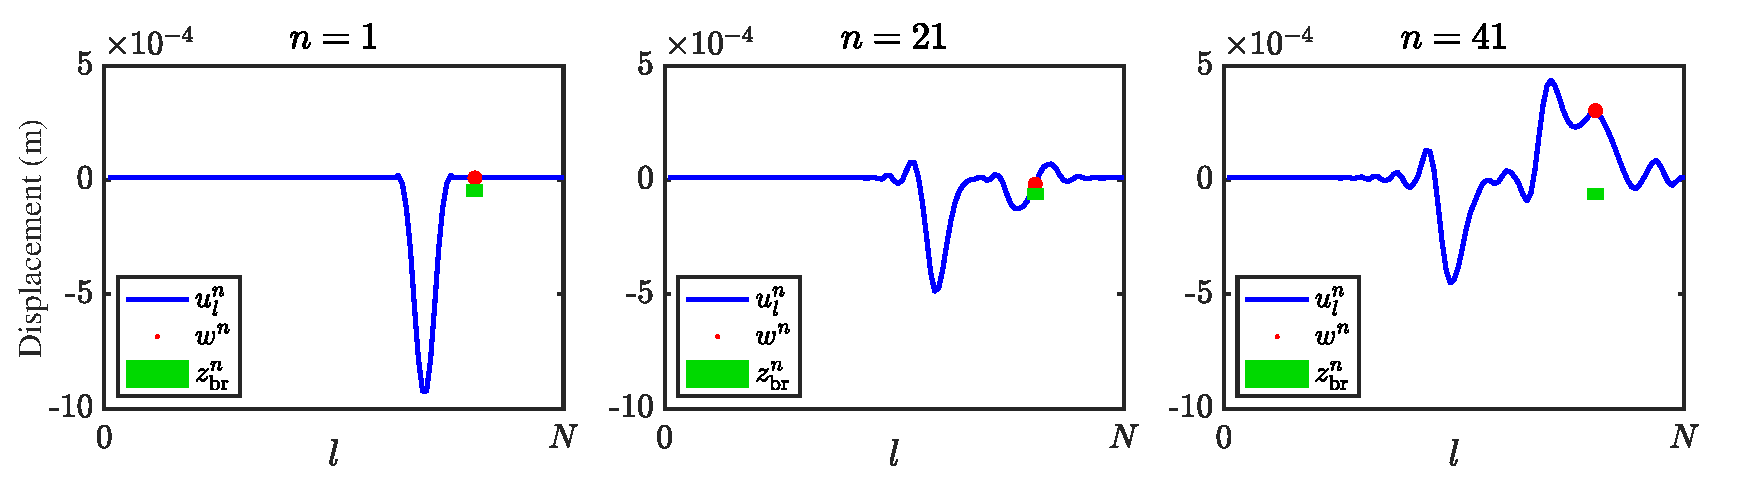
\includegraphics[width=\textwidth]{figures/contributions/tromba/trombaExcite.eps}
    \caption{The string of the tromba marina (blue) excited using a raised cosine. The string-mass interaction forces the mass (red) downwards which collides with the plate (green). \label{fig:trombaExcite}}
\end{figure}

\subsection{Energy analysis}
Using the energy analysis techniques presented in Section \ref{sec:energyAnalysis}, the total energy of the system can be shown to be of the following form:
\begin{equation}
    \dtp\left(\h_\stxt + \h_\mtxt + \h_\ptxt + \h_\sm + \h_\mp\right) = -\q_\stxt - \q_\mtxt - \q_\ptxt - \q_\Btxt - \p_\Btxt.
\end{equation}
Here, the total energy of the string is (Eq. \eqref{eq:energyBalanceStiffString}),
\begin{equation*}
    \begin{gathered}
        \h_\stxt = \frac{\rho_\stxt A}{2}\lVert\dtm \uln\rVert^2_{d_\stxt} + \frac{T}{2}\langle\dxp\uln, e_{t-}\dxp\uln\rangle_{\underline{d_\stxt}} + \frac{E_\stxt I}{2}\langle\dxx\uln, e_{t-}\dxx\uln\rangle_{\overline{\underline{d_\stxt}}}\ ,
    \end{gathered}
\end{equation*}
the total energy of the mass is (Eq. \eqref{eq:energyBalanceMassSpringDamper}) 
\begin{equation*}
    \h_\mtxt = \frac{M}{2}(\dtm w^n)^2 + \frac{K}{2}w^n e_{t-}w^n,
\end{equation*}
and the total energy of the plate is (Eq. \eqref{eq:energyBalanceThinPlate})
\begin{equation*}
    \h_\ptxt = \frac{\rho_\ptxt H}{2} \left\lVert\delta_{t-}\zlmn\right\rVert_{d_\ptxt}^2 + \frac{D}{2}\langle\dDelta \zlmn, e_{t-}\dDelta \zlmn\rangle_{\overline{\underline{d_\ptxt}}}\ .
\end{equation*}
The energy of the string-mass connection and the mass-plate collision are (Eq. \eqref{eq:collisionEnergy})
\begin{equation*}
    \h_\sm = \frac{(\psi_\sm^{n-1/2})^2}{2}, \qaq \h_\mp = \frac{(\psi_\mp^{n-1/2})^2}{2},
\end{equation*}
respectively.

The damping terms are defined for the string as (Eq. \eqref{eq:dampingTermStiffString})
\begin{equation*}
    \q_\stxt = 2\szX[\stxt] \rho_\stxt A \lVert\dtd\uln\rVert_{d_\stxt}^2 - 2 \soX[\stxt] \rho_\stxt A \langle \dtd \uln, \dtm \dxx \uln \rangle_{d_\stxt},
\end{equation*}  
for the mass as (Eq. \eqref{eq:massDampingEnergy})
\begin{equation*}
    \q_\mtxt = R\left(\dtd w^n \right)^2
\end{equation*}
and the plate as
\SWcomment[need to write still...]

Finally, the power dissipated and the supplied by the bow are defined as (Eq. \eqref{eq:energyBalanceBow})
\begin{equation*}
    \q_\Btxt =  f_\Btxt^n \Phi(\vrel^n) \vrel^n \qaq \p_\Btxt = f_\Btxt^n \Phi(\vrel^n)v_\Btxt^n,
\end{equation*}
respectively. 

Figure \ref{fig:trombaEnergy} shows the plots of the energy for an implementation of the tromba marina presented in this chapter without losses. The system is excited with a raised cosine for clarity of the figures and plots correspond to the system states shown in Figure \ref{fig:trombaExcite}.

% \begin{equation*}
    
% \end{equation*}

\begin{figure}[h]
    \centering
    \begin{tikzpicture}[->,node distance=3cm,
        thick,main node/.style={circle,draw}]
    
        \node[] (image) at (0,0) {
        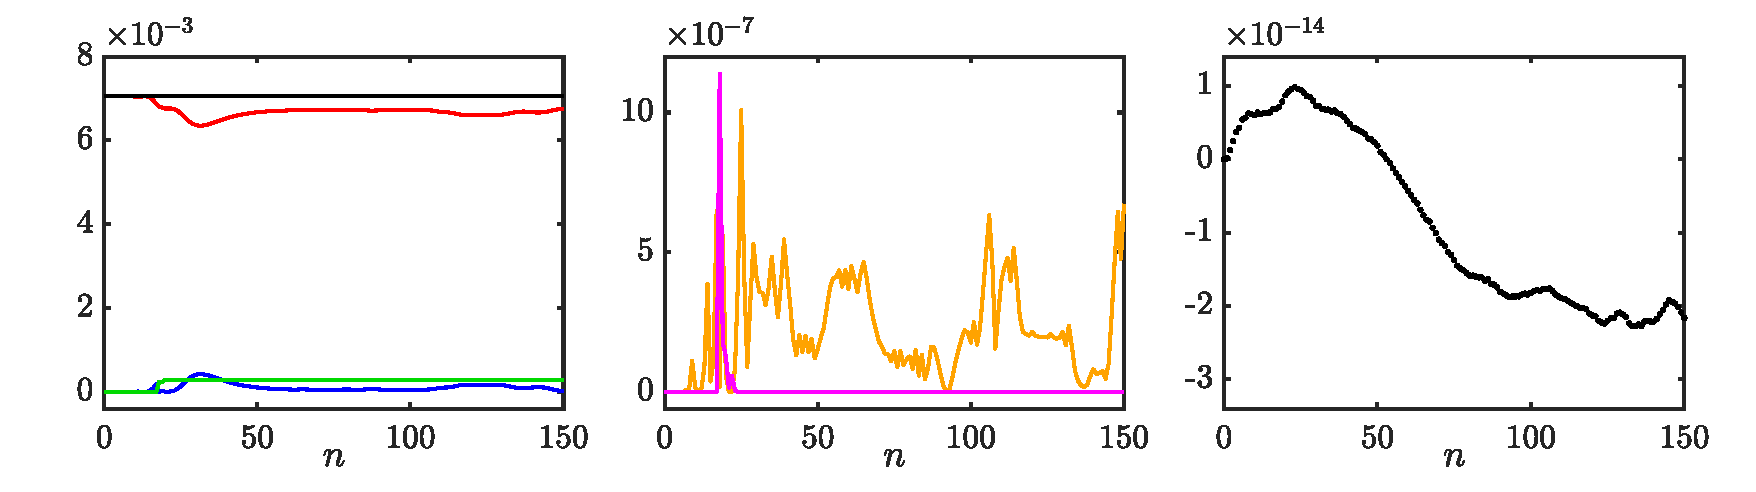
\includegraphics[width=\textwidth]{figures/contributions/tromba/trombaEnergy.eps}
        };
    
        \def\xLoc{-6}
        \node[] (h) at (\xLoc, 1) {\small $\mathfrak{h}_\text{tot}$};
        \node[] (s) at (\xLoc, 0.5) {\small $\color{blue}\mathfrak{h}_\stxt$};
        \node[] (m) at (\xLoc, 0) {\small $\color{red}\mathfrak{h}_\mtxt$};
        \node[] (p) at (\xLoc, -0.5) {\small $\color[HTML]{00DB00}\mathfrak{h}_\ptxt$};
        
        \node[] (c1) at (-0.7, 1.1) {\small $\color[HTML]{FF00FF}\mathfrak{h}_\mp$};
        \node[] (c2) at (1, 0.5) {\small $\color[HTML]{FFA400}\mathfrak{h}_\sm$};

        \node[] (he) at (2, 0.5) {\small $\mathfrak{h}_\text{e}$};
      \end{tikzpicture}
      \caption{The energy of the tromba marina excited with a raised cosine (see Figure \ref{fig:trombaExcite}). The left panel shows the total energy (black) present in the system as well as the energy of the string (blue), mass (red) and plate (green) respectively. The second panel shows the energy of the mass-plate (magenta) and string-mass (orange) interactions and the right panel shows the normalised energy (according to Eq. \eqref{eq:normalisedEnergy}) and shows that the deviation of the energy is within machine precision. \label{fig:trombaEnergy}}
\end{figure}
\section{Real-Time Implementation}
\SWcomment[not so sure if I should include more. Chapter might be done..]
\subsection{Considerations}
No bowing at the bridge.

To prevent the system from getting more complex, it is assumed that the bow will not interact with the bridge location. 

\subsection{Control using Sensel Morph}

\subsection{VR Application}
